%%%%%%%%%%%%%%%%%%%%%%%%%%%%%%%%%%%%%%%%%
% University/School Laboratory Report
% LaTeX Template
% Version 3.1 (25/3/14)
%
% This template has been downloaded from:
% http://www.LaTeXTemplates.com
%
% Original author:
% Linux and Unix Users Group at Virginia Tech Wiki 
% (https://vtluug.org/wiki/Example_LaTeX_chem_lab_report)
%
% License:
% CC BY-NC-SA 3.0 (http://creativecommons.org/licenses/by-nc-sa/3.0/)
%
%%%%%%%%%%%%%%%%%%%%%%%%%%%%%%%%%%%%%%%%%

%----------------------------------------------------------------------------------------
%	PACKAGES AND DOCUMENT CONFIGURATIONS
%----------------------------------------------------------------------------------------

\documentclass{article}

\usepackage{graphicx}
\usepackage{caption}
\usepackage{subcaption}

\usepackage[finnish]{babel} %ääkköset
\usepackage[utf8]{inputenc}
\usepackage[T1]{fontenc}

\usepackage[version=3]{mhchem} % Package for chemical equation typesetting
\usepackage{siunitx} % Provides the \SI{}{} and \si{} command for typesetting SI units
\usepackage{graphicx} % Required for the inclusion of images
\usepackage{natbib} % Required to change bibliography style to APA
\usepackage{amsmath} % Required for some math elements 

\setlength\parindent{0pt} % Removes all indentation from paragraphs

\renewcommand{\labelenumi}{\alph{enumi}.} % Make numbering in the enumerate environment by letter rather than number (e.g. section 6)

%\usepackage{times} % Uncomment to use the Times New Roman font

%----------------------------------------------------------------------------------------
%	DOCUMENT INFORMATION
%----------------------------------------------------------------------------------------

\title{Toteutusdokumentti: elektronirakenteen optimointi atomiorbitaalittomaan tiheysfunktionaaliteorian avulla} % Title

\author{Markus \textsc{Kaukonen} % Author name
}

\date{\today} % Date for the report


\begin{document}

\maketitle % Insert the title, author and date
\hspace{1cm} \texttt{email: markus.kaukonen@iki.fi, opiskelijanumero: 010974524}

\newpage
% If you wish to include an abstract, uncomment the lines below
% \begin{abstract}
% Abstract text
% \end{abstract}

%----------------------------------------------------------------------------------------


\section{Ohjelman yleisrakenne}
Ohjelma minimoi kokonaisenergiaa joko Monte Carlo (MC) tai Steepest
Descent (SD) menetelmällä. Minimointimenetelmä on kuvattu
määrittelydokumentissa. MC minimointiin liittyvät algoritmit ovat
paketissa 'laskentaa.py'. SD minimointiin liittyvät algoritmit ovat
paketissa 'laskentaa\_sd.py'.

Kokonaisenergia lasketaan määrittelydokumentissa kuvatulla
tavalla. Energian laskemiseen liittyvät funktiot ovat paketissa
'energiat.py'. Samassa paketissa lasketaan myös elektronien aiheuttama
Hartree potentiaali, joka iteroidaan Gauss-Seidel iteraatiolla (Gauss
Seidel iteraatio sijaitsee paketissa 'laskentaa.py').

Alkuarvot luetaan tiedostoista jotka on nimetty pääohjelmassa
'vertaile\_nopeuksia.py'. Luentarutiinit ovat pakkauksessa
'read\_data.py'.

Elektronitiheydet, Hartree potentiaali ja energian
funktionaaliderivaatta tiheyden suhteen esitetään kolmi- tai
kaksiulotteisissa grideissä. Gridiobjekti on määritelty paketissa
'gridi.py'.

Tässä työssä pääohjelma 'vertaile\_nopeuksia.py' tekee energian
minimoinnin kolmelle eri 2d-systeemille (input tiedostot:
'alkuarvot.txt\_5x5x0', 'alkuarvot.txt\_10x10x0',
'alkuarvot.txt\_16x16x0'). Minimointi tehdään sekä monte carlo
menetelmällä että steepest descent menetelmällä. Lisäksi minimoidusta
elektronitiheydestä piirretään kuva (piirtorutiineja on paketissa
'piirtoa.py'.


\section{Suorituskykyvertailu}
Työssä tehtiin minimointia kahdella eri menetelmällä (MC ja
SD). Allaolevassa taulukossa on esitetty minimoitu energia ja
minimointiin kulunut aika systeemin koon funktiona.  Laskenta tehtiin
ACER aspire (vm. 2010) kannettavalla tietokoneella (Intel(R) Core(TM)
i3-2310M CPU @ 2.10GHz). Systeemien koot pienimmästä suurimpaan ovat
5x5, 10x10 ja 16x16 gridipistettä. Atomiytimet on sijoitettu kohtiin:
5x5: ([2,2, varaus +1]), 10x10: ([2,2,+1],[2,4,+1],[8,7,+2], 16x16:
([3,3,+1],[8,2,+1]).
\begin{center}
\begin{table}
  \begin{tabular}{ | l | c | c | r |}
    \hline
    systeemi & menetelmä & Cpu [s] & Energia [H] \\
    \hline
    \hline
    pieni & MC & 0.6 & 1174.54 \\ \hline
    keski & MC & 27.6 & 3178.85 \\ \hline
    suuri & MC & 535.2 & 329.98 \\ \hline
    pieni & SD & 16.8 & 1174.47 \\ \hline
    keski & SD & 338 & 3169.44 \\ \hline
    suuri & SD & 26560 & 320.49 \\ \hline
    \hline
  \end{tabular}
\caption[]{Verrataan monte carlo (MC) ja steepest descent SD
  minimointien kuluttamia Cpu-aikoja ja saatua energian minimiarvoa.}
\label{table:tulos1}
\end{table}
\end{center}
Taulukosta havaitaan että MC minimointi oli näissä systeemeissä
huomattavasti nopeampi minimointimenetelmä. Toisaalta SD-menetelmä
onnistui löytämään energiaminimin paremmin.

Kuvissa \ref{fig:mc-simulaatiot} ja \ref{fig:sd-simulaatiot} on
esitetty konvergoituneet elektronitiheydet eri systemeille joko MC-
tai SD-minimoitien tuloksena. Havaitaan että ne ovat kvalitatiivisesti
samankaltaisia, mikä olikin tämän työn tavoitteena. Lisäksi
elektronitiheys on keskittynyt ytimien läheisyyteen, joten voidaan
päätellä että tulokset ovat fysikaalisesti mielekkäitä.

\begin{figure}
        \centering
        \begin{subfigure}[b]{0.3\textwidth}
                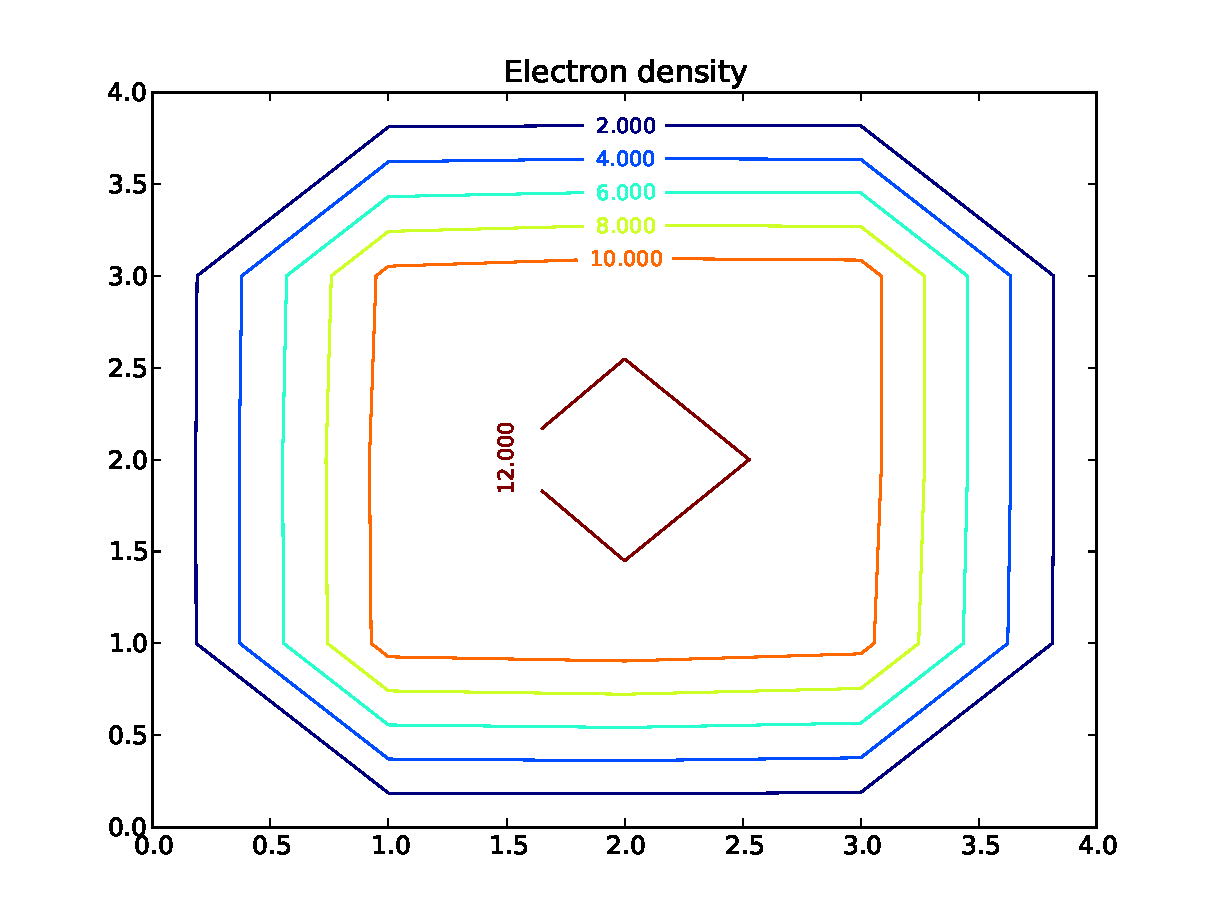
\includegraphics[width=\textwidth]{mc_pieni.pdf}
                \caption{MC: pieni}
                \label{fig:gull}
        \end{subfigure}%
        ~ %add desired spacing between images, e. g. ~, \quad, \qquad, \hfill etc.
          %(or a blank line to force the subfigure onto a new line)
        \begin{subfigure}[b]{0.3\textwidth}
                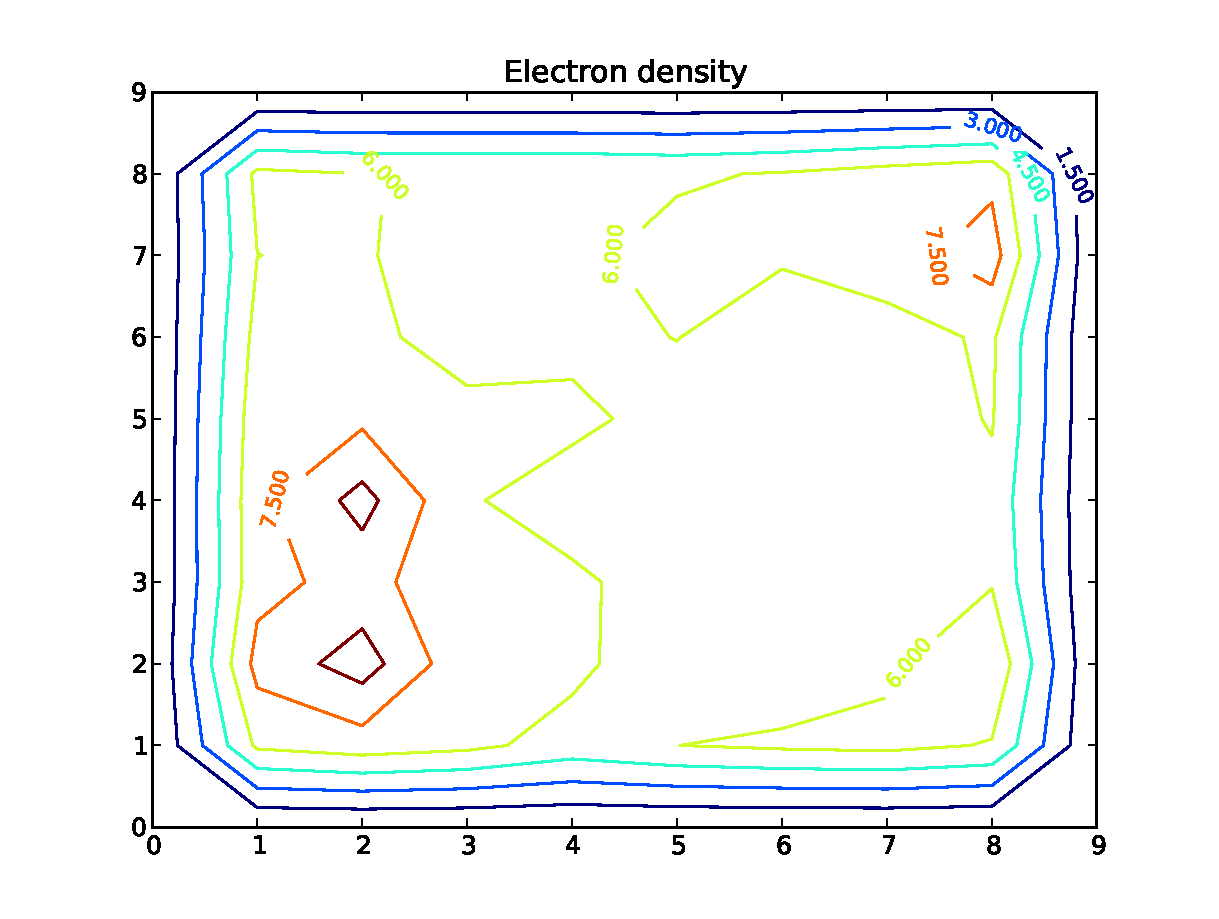
\includegraphics[width=\textwidth]{mc_keski.pdf}
                \caption{MC: keski}
                \label{fig:tiger}
        \end{subfigure}
        ~ %add desired spacing between images, e. g. ~, \quad, \qquad, \hfill etc.
          %(or a blank line to force the subfigure onto a new line)
        \begin{subfigure}[b]{0.3\textwidth}
                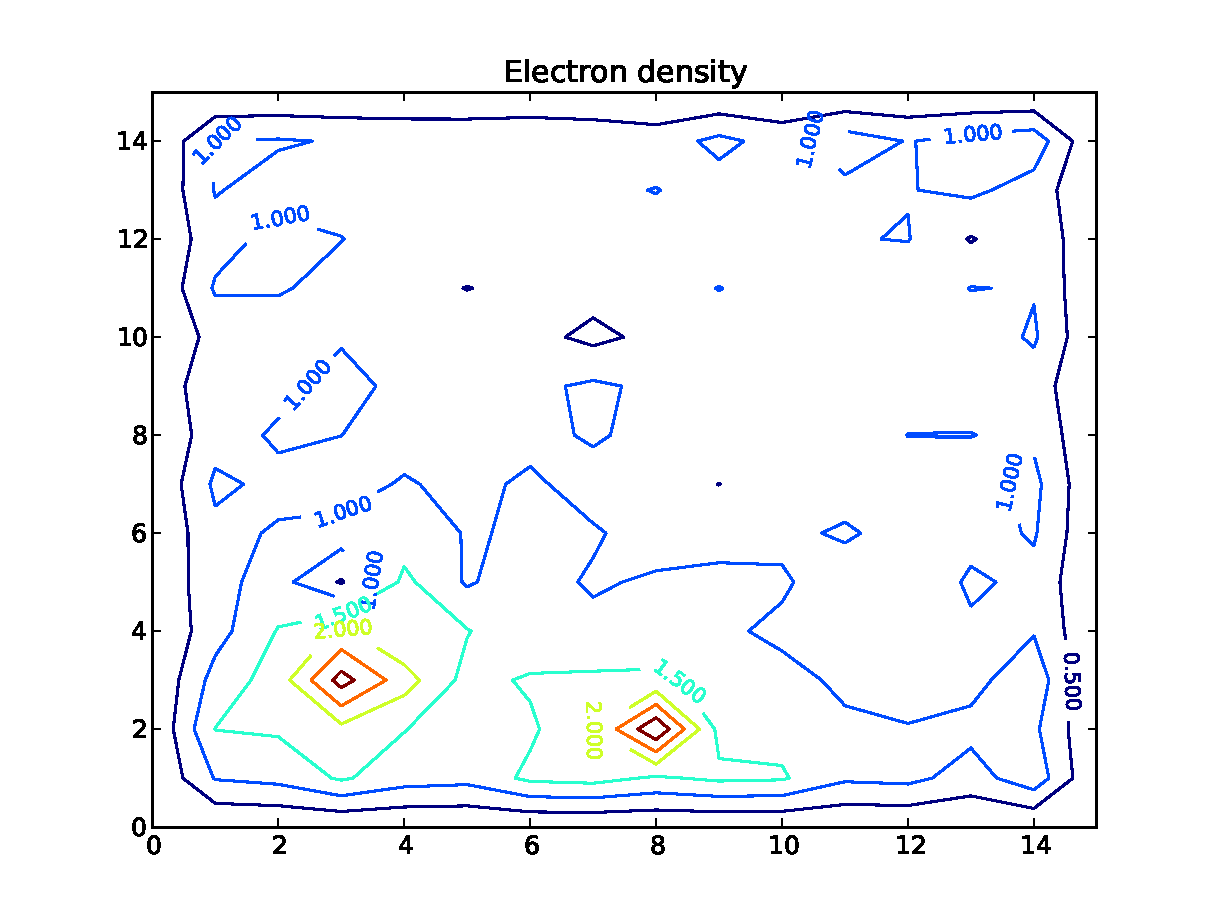
\includegraphics[width=\textwidth]{mc_suuri.pdf}
                \caption{MC: suuri}
                \label{fig:mouse}
        \end{subfigure}
        \caption{Monte Carlo (MC) simulointien tuottamia elektronitiheyksiä kolmessa testisysteemissä.}\label{fig:animals}
        \label{fig:mc-simulaatiot}.
\end{figure}

\begin{figure}
        \centering
        \begin{subfigure}[b]{0.3\textwidth}
                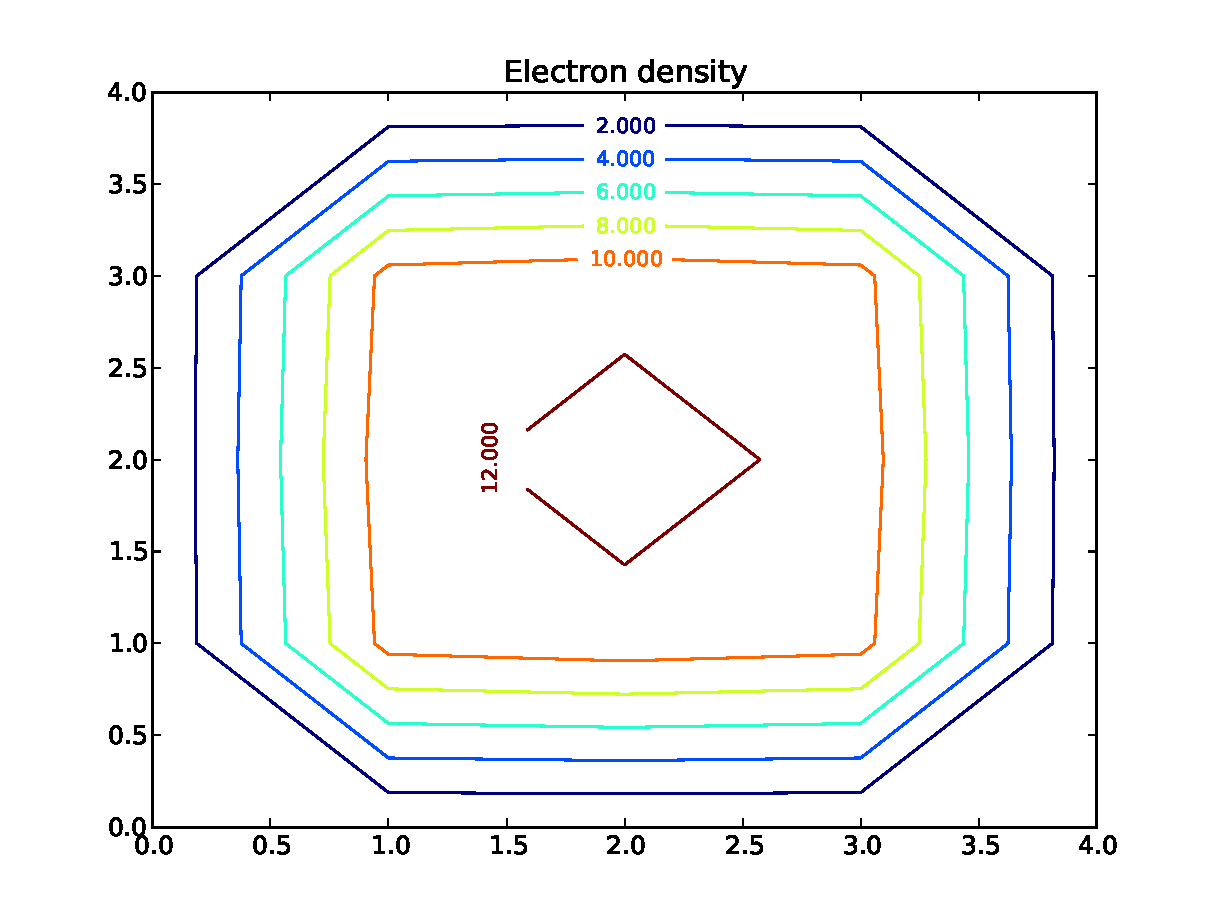
\includegraphics[width=\textwidth]{md_pieni.pdf}
                \caption{SD: pieni}
                \label{fig:gull}
        \end{subfigure}%
        ~ %add desired spacing between images, e. g. ~, \quad, \qquad, \hfill etc.
          %(or a blank line to force the subfigure onto a new line)
        \begin{subfigure}[b]{0.3\textwidth}
                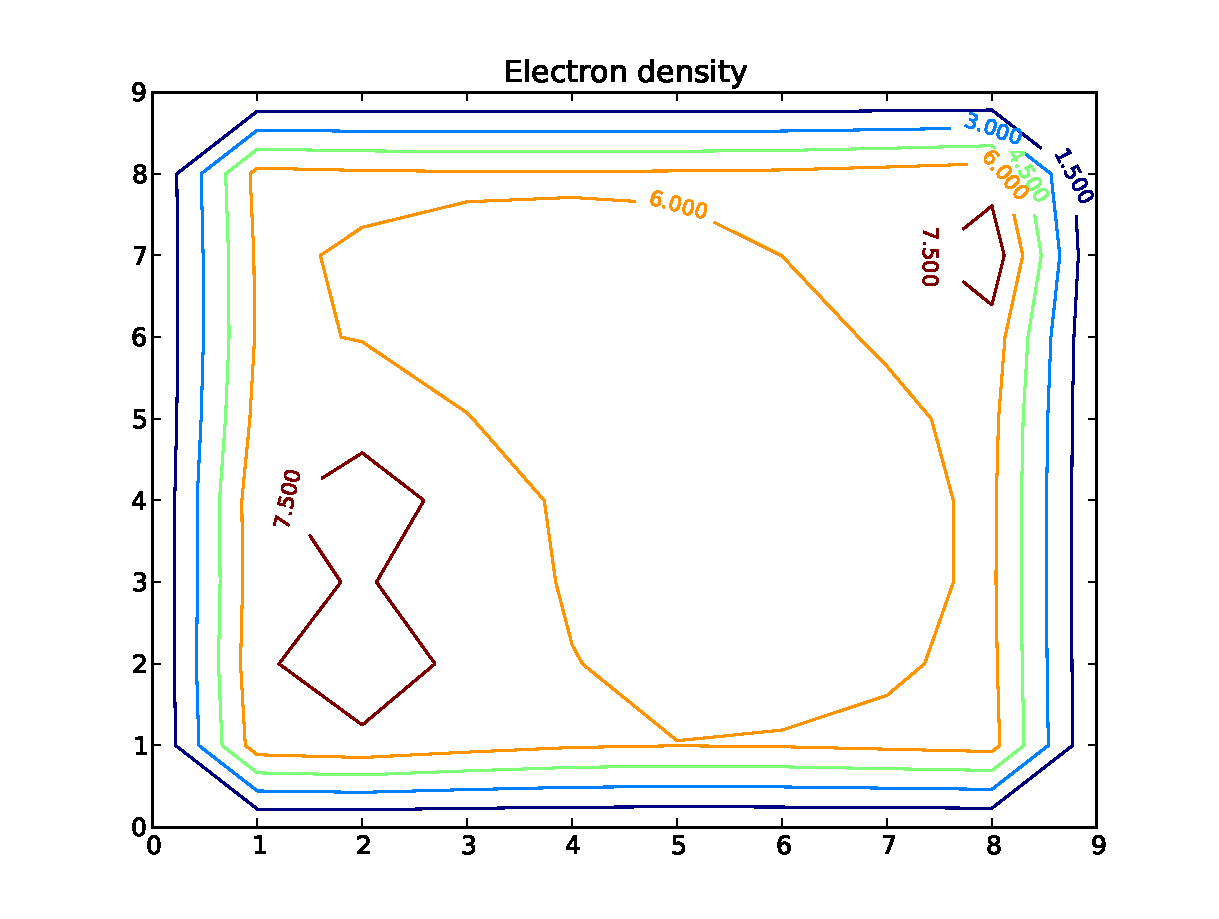
\includegraphics[width=\textwidth]{md_keski.pdf}
                \caption{SD: keski}
                \label{fig:tiger}
        \end{subfigure}
        ~ %add desired spacing between images, e. g. ~, \quad, \qquad, \hfill etc.
          %(or a blank line to force the subfigure onto a new line)
        \begin{subfigure}[b]{0.3\textwidth}
                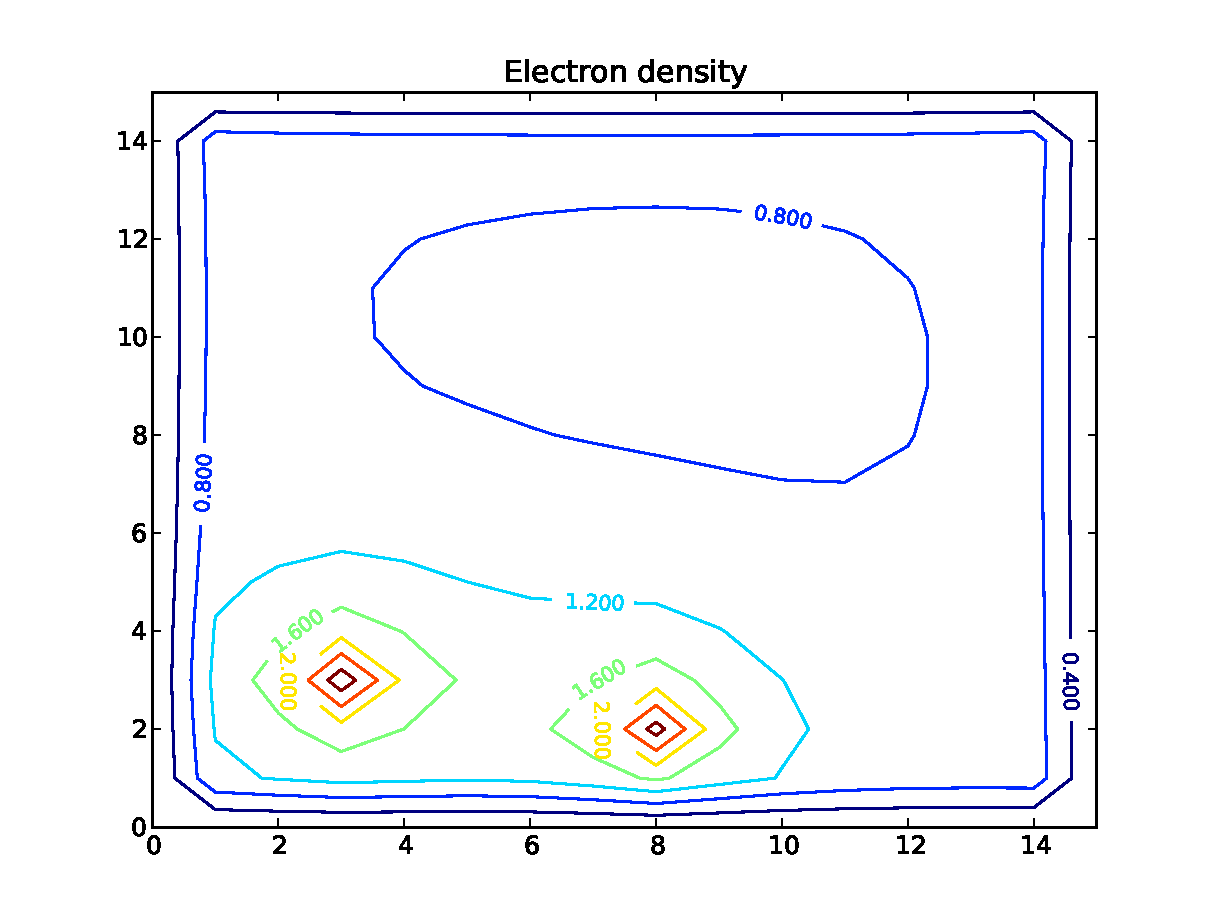
\includegraphics[width=\textwidth]{md_suuri.pdf}
                \caption{SD: suuri}
                \label{fig:mouse}
        \end{subfigure}
        \caption{Steepest Descent (SD) simulointien tuottamia elektronitiheyksiä kolmessa testisysteemissä.}\label{fig:animals}
        \label{fig:sd-simulaatiot}
\end{figure}

\begin{figure}[h]
\begin{center}
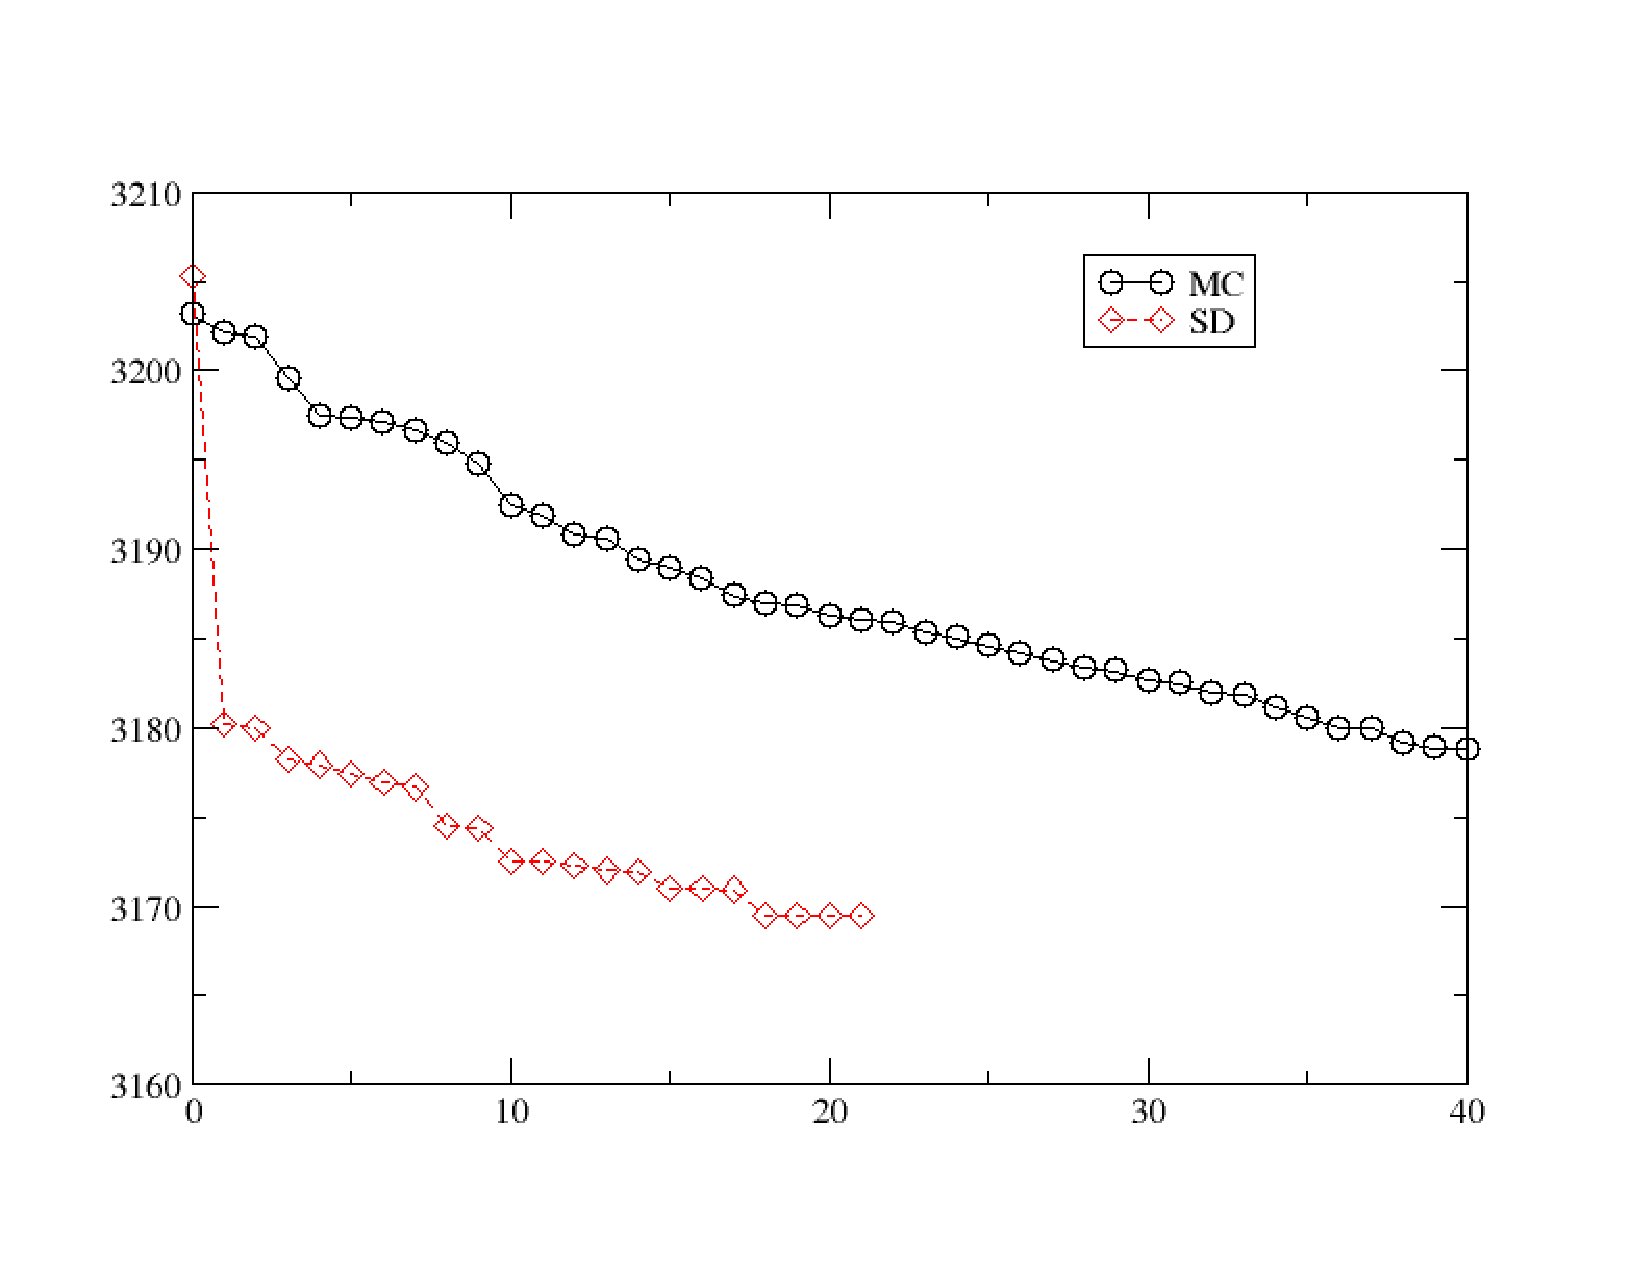
\includegraphics[width=0.65\textwidth]{keski_konvergenssi.pdf} % Include the image placeholder.png
\caption{Kokonaisenergian konvergoiminen iteraatioaskelten
  funktiona. Input file oli 'alkuarvot.txt\_10x10x0'. 'SD' tarkoittaa
  että minimointi tehtiin Steepest descent menetelmällä ja 'MC' että
  minimointiin Monte Carlo algoritmilla.}
\label{fig:konvergenssit}
\end{center}
\end{figure}


Kuvissa \ref{fig:konvergenssit} on esitetty energian konvergoituminen
minimointiaskeleiden funktiona. Havaitaan että MC minimointi tuottaa
liian korkean kokonaisenergian. Tämä saattaa johtua siitä että energia
katsottiin konvergoituneeksi jos energian muutos oli pienempää kuin
$10^{-4}$ H. Varmempi tapa olisi ollut vaatia että energian muutos
olisi ollut pienempää kuin $10^{-4}$ H esimerkiksi viiden
minimointiaskelen ajan. Toinen mahdollinen syy MC-minimoinnin
huonompaan suoritumiseen voi olla MC-minimoinneissa käytetty
lämpötila. Tässä työssä käytettiin lämpötilaa 100 K. Korkeampaa
lämpötilaa käyttämällä olisi todennäköisesti paremmin voitu välttää
paikalliset energiaminimit.

\section{Työn mahdolliset puutteet ja parannusehdotukset}
Ensinnä täytyy sanoa että muutamassa viikossa ei saada aikaakn
täydellistä kvanttikemian ohjelmaa. Tässä työssä saatiin aikaan sopiva
lähtökohta myöhemmälle mahdolliselle kehitystyölle.

Energan minimointia tulisi parantaa jotta globaali minimointi
löydetään mahdollisimman hyvin. Tämä onnistuu tehokkaimin ja
helpoimmin käyttämällä Scipy:n valmiiita
minimointirutiineita[\cite{jones2001scipy}]. Nyt etenkin rajoitettu
optimointi (elektronimäärän piti säilyä vakiona) aiheutti ongelmia
minimoinnneissa.

Toinen puute ohjelman tämänhetikisessä versiossa on se että kaikki
elektronit optimoidaan samanaikaisesti. Muutama vuosi sitten on saatu
selville että tulokset orbitaalivapaassa tiheysfukntionaaliteoriassa
paranevat huomattavasti jos eri kulmaliikemäärän omaavat elektronit
optimoidaan erikseen[\cite{ke2013angular}].

\section{Javadocia vastaava dokumentaatio}
Javadocia vastaava dokumentaatio on toteutettu Sphinx:illä.  Se
käynnistyy selaimella esim. komennolla 'firefox
TiraLabra/Docs/html/index.html'


%----------------------------------------------------------------------------------------
%	BIBLIOGRAPHY
%----------------------------------------------------------------------------------------

\bibliographystyle{apalike}

\bibliography{Maarittelydokumentti}


\end{document}
